%!TEX TS-program = xelatex

\documentclass[12pt]{report}
\usepackage[english]{babel}
\usepackage{uis-thesis} % Options: print
\usepackage[colorlinks]{hyperref}
\usepackage[utf8]{inputenc}
\usepackage{natbib}
\usepackage[printonlyused,withpage]{acronym}
\usepackage{refcount}% required for \getpagerefnumber
\usepackage{xr}% required to reference labels in external documents
\usepackage{listings}
\usepackage{color}

\definecolor{dkgreen}{rgb}{0,0.6,0}
\definecolor{gray}{rgb}{0.5,0.5,0.5}
\definecolor{mauve}{rgb}{0.58,0,0.82}

\hypersetup{
    colorlinks=true,
    linkcolor=blue,
    filecolor=magenta,      
    urlcolor=cyan,
    pdftitle={Overleaf Example},
    pdfpagemode=FullScreen,
    }

\lstset{frame=tb,
  language=Java,
  aboveskip=3mm,
  belowskip=3mm,
  showstringspaces=false,
  columns=flexible,
  basicstyle={\small\ttfamily},
  numbers=none,
  numberstyle=\tiny\color{gray},
  keywordstyle=\color{blue},
  commentstyle=\color{dkgreen},
  stringstyle=\color{mauve},
  breaklines=true,
  breakatwhitespace=true,
  tabsize=3
}


% UiS recommends Georgia for the body text, but you are free to use another
% font for the body text; if you want to use another font just e this line.
\setmainfont{Georgia}

% Optional: specify path to photo
%\photo{photos/ide}
% Optional: credit the photographer; required for many photos; you must check
%\photocredit{Hein Meling}
\title{NFT as a proof of Digital Ownership-reward system integrated to a Secure Distributed Computing Blockchain Framework}
\authors{Asahi Cantu}
\department{ide}
\date{June 2022}

% Optional: uncomment if you want to display faculty name as well
\faculty{tn}
% Allowed values: bachelor, master, phd, tr
\reporttype{master}
% \reporttype[404]{phd}
% Allowed values: cs, ds, ee, medtek
\specialization{cs}
% Use only for phd thesis
% \isbn{000-00-0000-000-0}
% \issn{0000-0000}
% Uncomment only if your thesis has been granted restricted access
% \restricted

%-----------------------------------------------------------------
\begin{document}
% Values: 1-9 select different color schemes, 10 for draft versions (to save ink)
\uiscover{4}
\frontmatter
\pagestyle{empty} 
\declaration

\input{frontmatter/quote}
\input{frontmatter/abstract}
\input{frontmatter/ack}

\tableofcontents

% Abbreviations, use \ac{NFT} to map them from the document
\section{Abbreviations}

\begin{acronym}
    \acro{API}{Application Program Interface}
    \acro{AWOL}{Absence Without Official Leave}
    \acro{BFT}{Byzantine Fault Tolerance}
    \acro{CA}{Certificate Authority}
    \acro{CFT}{Crash Fault Tolerant}
    \acro{CID}{Content Identifier}
    \acro{CPU}{Central Processing Unit}
    \acro{DAC}{Decentralized Autonomous Corporation}
    \acro{DAG}{Directed Acyclic Graph}
    \acro{DAO}{Decentralized Autonomous Organization}
    \acro{DAPP}{Decentralized Application}
    \acro{DeFi}{Decentralized Finance}
    \acro{DFS}{Distributed File System}
    \acro{DLT}{Distributed Ledger Technology}
    \acro{DMS}{Data Management System}
    \acro{DSL}{Domain-specific Language}
    \acro{EIP}{Ethereum Improvement Proposals}
    \acro{ERC}{Ethereum Request for Comments}
    \acro{EHR}{Electronic Health Records}
    \acro{ETH}{Ethereum Cryptocurrency token}
    \acro{FT}{Fungible Token}
    \acro{IPFS}{Interplanetary File System}
    \acro{IT}{Information Technology}
    \acro{IoT}{Internet of Things}
    \acro{IPS}{Instructions Per Second}
    \acro{kB}{KiloByte}
    \acro{KB}{KiloByte}
    \acro{KYC}{Know Your Customer}
    \acro{MiB}{Mebibyte}
    \acro{MPA}{Multi-party authorization} 
    \acro{NFT}{Non Fungible Token}
    \acro{Nonce}{Number only used once}
    \acro{OS}{Operating System}
    \acro{PBFT}{Practical Byzantine Fault Tolerance}
    \acro{PKI}{Public Key Infrastructure}
    \acro{PoA}{Proof of Authority}
    \acro{PoET}{Proof of Elapsed Time}
    \acro{PoS}{Proof of Stake}
    \acro{PoW}{Proof of Work}
    \acro{P2P}{Peer-to-Peer}
    \acro{REST}{Representational State Transfer}
    \acro{s}{Seconds}
    \acro{TB}{TeraByte}
    \acro{TCG}{Trading Card Game}
    \acro{TPS}{Transactions Per Second}
    \acro{UAV}{Unmanned Aerial Vehicle}
    \acro{UI}{User Interface}
    \acro{USD}{United States Dollar}
    \acro{WSL}{Windows Subsystem for Linux}
\end{acronym}

    
    % \input{frontmatter/symbols}
%-----------------------------------------------------------------
\mainmatter
% Begin normal, numeric (1,2,3...) page numbering
\input{chapters/00-intro/00-intro-00-main}
\input{chapters/00-intro/00-intro-01-background}
\input{chapters/00-intro/00-intro-02-objectives}
\input{chapters/00-intro/00-intro-03-approach}
\input{chapters/00-intro/00-intro-04-outline}

\input{chapters/01-related/01-related-00-Main}
\input{chapters/01-related/01-related-01-Blockchain}
\input{chapters/01-related/01-related-02-Hyperledger}
\input{chapters/01-related/01-related-03-IPFS}
\input{chapters/01-related/01-related-04-SimilarSystems}

\input{chapters/02-approach/02-approach-00-main}
\input{chapters/02-approach/02-approach-01-intro-00-main}
\input{chapters/02-approach/02-approach-01-intro-01-blockchain}
\input{chapters/02-approach/02-approach-01-intro-02-SmartContracts}
\input{chapters/02-approach/02-approach-01-intro-03-Hyperledger}
\input{chapters/02-approach/02-approach-01-intro-04-IPFS}

\input{chapters/02-approach/02-approach-02-existing-00-main}
%!TEX root = ../../main.tex
\section{Analysis}

Ever since the world has been interconnected over the Internet, malicious parties have intended to take advantage over their computational resources and digital assets. As technologies improve and the society evolves into a digital world, attacks become more sophisticated, frequent and devastating. It is increasing month by month in an exponential ways, compromising governments and companies systems and data. 

Such has been the risk and consequences of cyber attacks and data breaches that in 2021\cite{10DataBreaches:online}:
\begin{enumerate}
    \item On average a data breach costs up to 8.64 million \ac{USD}.
    \item Global Cybercrime costed over 6 trillion
    \item Businesses fell victim of ransomware every 11 seconds.
    \item Took up to 220 days to contain a data breach, with healthcare industry being the slowest to recover with over 320 days.
    \item  As more users perform remote works cybercriminals keep increasing their attacks over telecommuters and remote access pathways
    \item Properly containing a data breach could have saved up to 1 million \ac{USD} in less than 200 days
    \item More than 8\ac{TB} of data were leaked.
    \item A total of 270 major data breaches occurred, exposing 238 Million of records and 16 billion \ac{USD} per day.
\end{enumerate}

\begin{figure}[h]
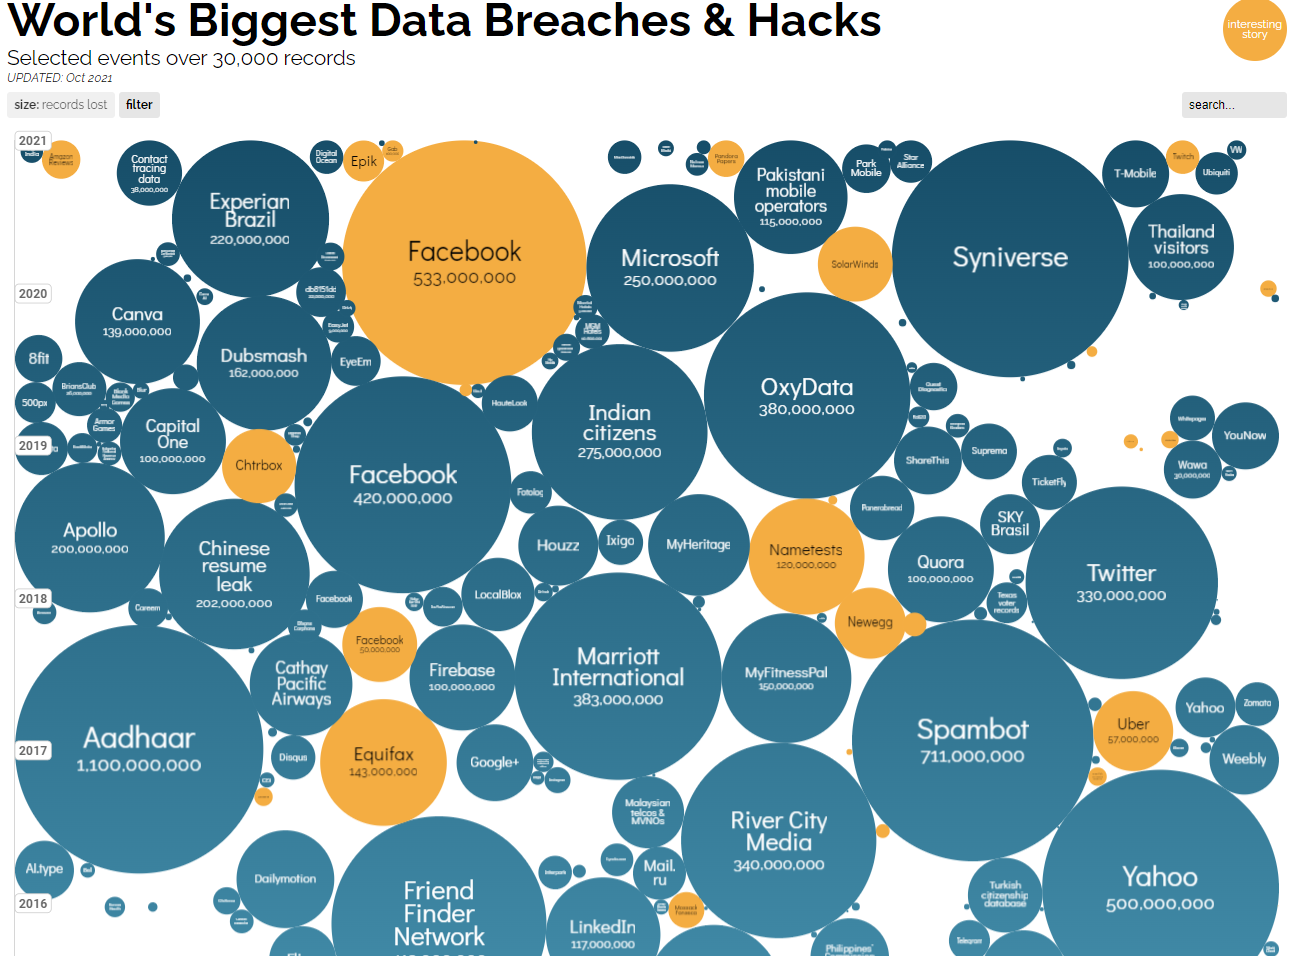
\includegraphics[width=15cm]{img/DataBreach.png}
s\caption{Word's Biggest data breaches and hacks occurred fro 2016 to October 2021  \cite{WorldDataBreach:online}}
\label{fig:worldDataBreach}
\end{figure}
Moreover, in 2021 several Nordic companies were victim of important cyber attacks ,peaking in December 2021\cite{Nordicco81:online}. Affected industries corresponded to the region’s largest industrial, food and  service providing sector.
Affected companies were Vestas, Wind Systems, Amedia, Nortura
and Nordic Choice Hotels

\begin{figure}[h]
\includegraphics[width=15cm]{img/GDPRDataBreach.jpeg}
\centering
\caption{Top-10 GDPR-per-country data breaches notified per EEA jurisdiction from May 2018 to October 2020\cite{Statista:online}}
\end{figure}

It is clear that with the current resources (both human and digital) is impossible to overcome these threats. In addition data has become a vital asset. Companies are now legally liable to protect it and ensure that is properly protected with state of the art technologies. Failing to do that could lead them to bankruptcy or serious fines which in some cases could be of irrecoverable damage, lost of reputation or even catastrophic disasters for the society.


\subsubsection{Hypothesis}
\label{analysis_hyp}

With the implementation of a decentralized system in a Hyperledger Fabric and a chaincode implementing \ac{ERC}-721 standard with \ac{IPFS} network, it will be possible to manage and handle data between organizations in a safer and more secure way. Sharing information and ensuring that the non-repudation\footnote{\input{Footnotes/NonrepudationPrinciple}} principle remains consistent over the network no matter how many parties or users join the infrastructure. 
\input{chapters/02-approach/02-approach-04-proposed-00-main} 


\input{chapters/03-eval/03-eval-00-main}
%!TEX root = ../thesis.tex

\chapter{Discussion}
\label{ch:discussion}
The implementation of digital asset management through issuance of \ac{NFT}s represents a milestone in the generation of decentralized secure frameworks for industrial applications.

The implicit security of Blockchain with Hyperledger management and the privacy such technology offers will allow different organizations to participate and cooperate securely, but not anonymously. 

All parties will be able to acknowledge data ownership. If desired, data could be encrypted as well and managed trough additional smart contracts. In addition to this, \ac{IPFS} network is able to control, distribute and manage the added data as a \ac{DFS}. The final simulation of the environment allows testers, to acknowledge the workflow of the framework and further expand its capabilities in a modular way.

\section{Results}
The simulation was performed with the following operations:

\begin{enumerate}
    \item Minting NFT with Text data ~ 10KB
    \item Minting NFT with Image data ~ 200KB
    \item Minting NFT with Bin data ~ 100MB
    \item Minting NFT with a file of ~850MB
\end{enumerate}

The highest resource consuming process for the system is whenever data with high space resources is about to be minted. The communication with the server and IPFS network create a bottle neck in the simulation process and by running the resources locally.

\begin{table}[h!]
\begin{center}
\begin{tabular}{ |c|c|c|c|  }
 \hline
 \multicolumn{4}{|c|}{NFT Statistics} \\
 \hline
 No & File type & Size  & Elapsed time (s)\\
 \hline
 1   & Text     & 10KB &   0.5  \\
 2   & Image    & 200KB &   1.3 \\
 3   & PDF      & 100MB &   8.3 \\
 4   & Bin      & 850MB &   $\infty$ \\
 
 \hline
\end{tabular}
\caption{NFT Statistics.}
\label{table:NFTStats}
\end{center}
\end{table}

Whenever trying to mint an NFT File larger than 500 MB (previous tests were made with other files) the blockchain system, or at least the \ac{API} server takes significantly larger amount time than expected to submit the data. Although this might be a parameter or server side configuration, it certainly refrains users from submitting large amounts of information.

Final results of the built application indicate that it is potentially feasible to create decentralized systems specialized in data management and control for industrial purposes while dealing with chunks of data. For text data it is relatively easy to mint, submit and visualize under the IPFS Server.

\subsection{Infrastructure statistics}
The following statistics were performed by running \textit{docker stats} command where they where later on plotted.
\begin{figure}[h!]
        \centering
        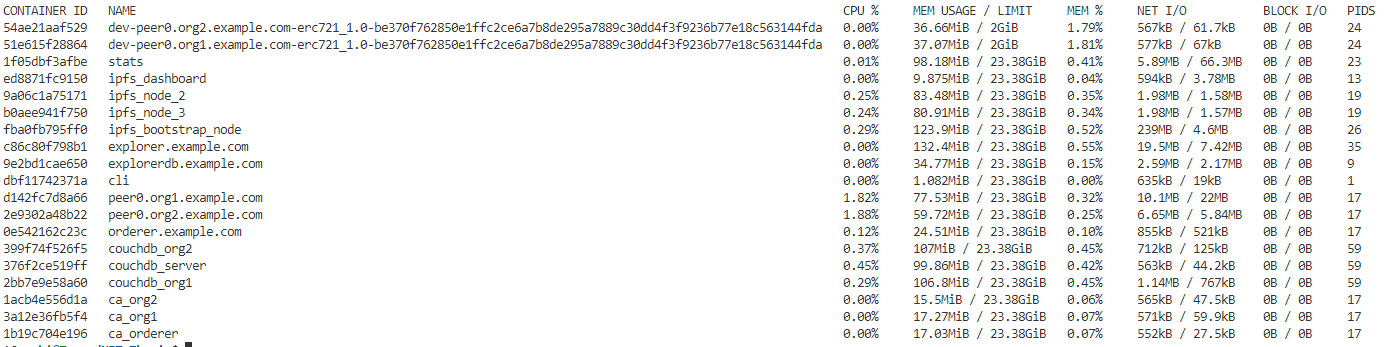
\includegraphics[width=15cm]{img/Docker_Stats.png}
        \caption{Docker statistics from current containers}
        \label{fig:dockerStats}
\end{figure}

\subsubsection{Memory Usage}
The image \ref{fig:dockerMem} shows the amount of memory used by all the servers. The containers with higher numbers are the ones used to provide statistics and insights. in Orange: The container to run statistics, whereas in blue the container running Hyperledger explorer \ac{UI}. The unit of measure has been performed in \ac{MiB}.
\begin{figure}[h!]
        \centering
        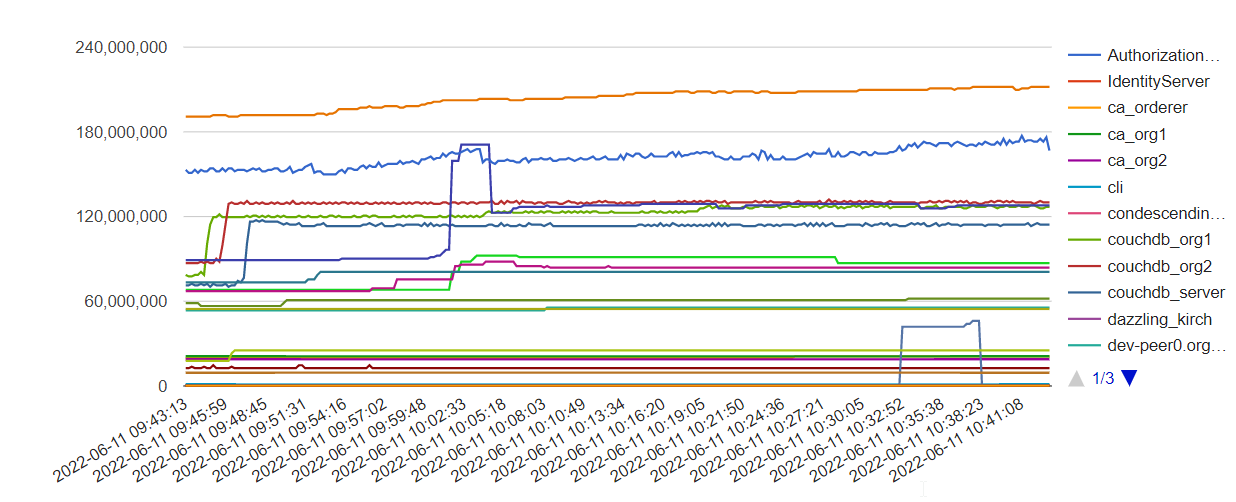
\includegraphics[width=15cm]{img/Docker_Mem.png}
        \caption{Infrastructure Memory Usage. Unit of measure in MiB}
        \label{fig:dockerMem}
\end{figure}

\subsubsection{CPU Usage}
Image \ref{fig:dockerCPU} shows the amount of \ac{CPU} in terms of \ac{IPS} executed. The peaks shown correspond to the IPFS network.
\begin{figure}[h!]
        \centering
        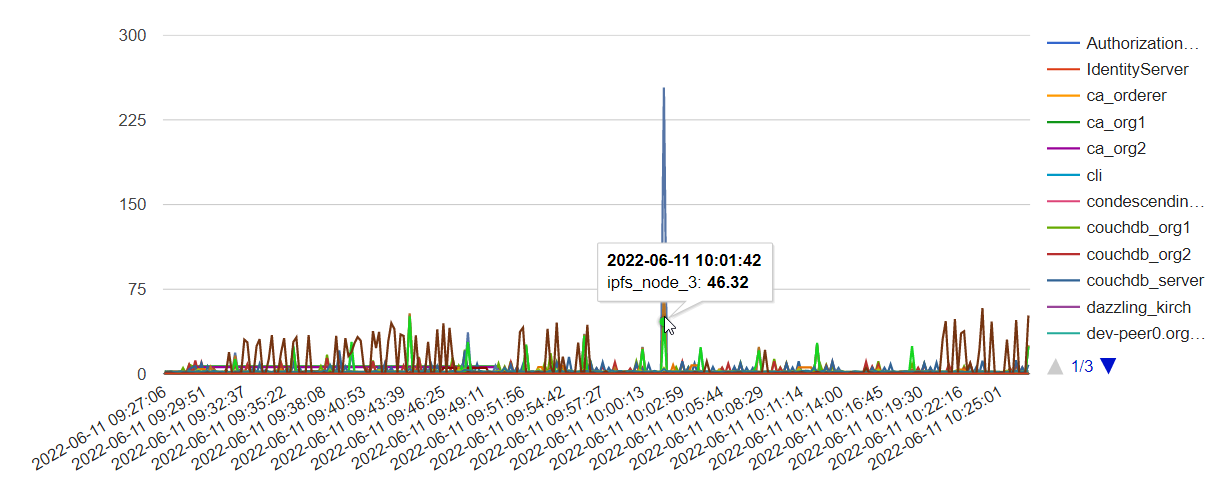
\includegraphics[width=15cm]{img/Docker_CPU.png}
        \caption{Infrastructure CPU Usage in IPS}
        \label{fig:dockerCPU}
\end{figure}

\subsubsection{Network inputs}
Image \ref{fig:dockerNetIn} shows all  network inputs consumed by each container. In color blue it can be highlighted that IPFS network is the node taking most of the network inputs due to the amount of memory consumed after minting large file sizes for the \ac{NFT}. Unit of measure is in \ac{kB}
\begin{figure}[h!]
        \centering
        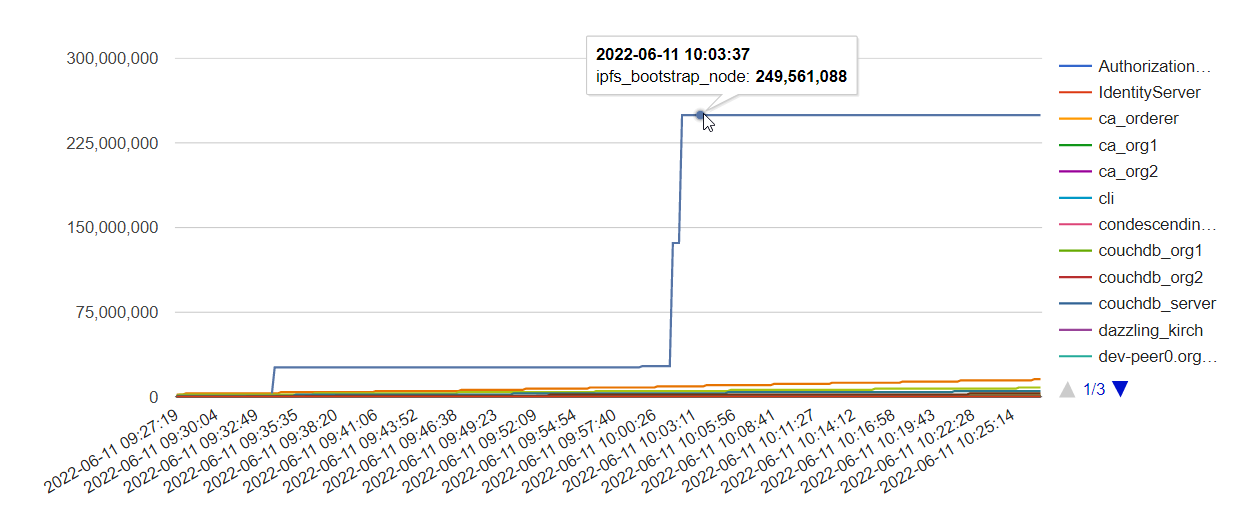
\includegraphics[width=15cm]{img/Docker_NetIn.png}
        \caption{Network Inputs}
        \label{fig:dockerNetIn}
\end{figure}

\subsubsection{Network outputs}
Image \ref{fig:dockerNetOut} shows all network outputs sent by each container. At the top the container used to run the statistics has the most of data sent. In In second place the peer node corresponding to organization one presents the one with the most information transmitted. Unit of measure is in \ac{kB}.
\begin{figure}[h!]
        \centering
        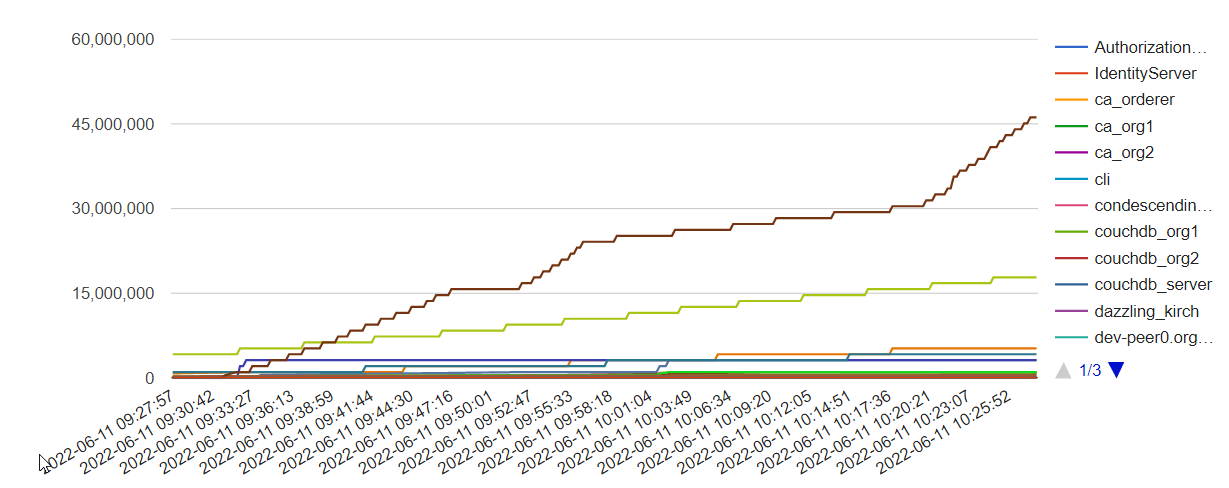
\includegraphics[width=15cm]{img/Docker_NetOut.png}
        \caption{Network Outputs}
        \label{fig:dockerNetOut}
\end{figure}



\subsection{Benchmarking and Blockchain metrics evaluation}
Hyperledger framework has a benchmark tool used to measure the performance and behavior of the blockchain, test it and evaluate it under stress scenarios to check its latency and behaviour under heavy usage. Tables \ref{table:Benchmark1} and \ref{table:Benchmark2} show the results thrown in raw data. Figure \ref{fig:CaliperBenchmark} presents relevant information about the usage and network stress results. as an HTML report, which is also available at:
\url{https://htmlpreview.github.io/?https://raw.githubusercontent.com/asahicantu/NFT-Thesis/main/caliper-benchmarks/report.html} Units of measure for the data are in \ac{s} and \ac{TPS}.

\begin{table}[h!]
\begin{center}
\begin{tabular}{ |c|c|c|c|c|c|  }
 \hline
 \multicolumn{6}{|c|}{Blockchain benchmark Part I.} \\
 \hline
 Name & Succ  & Fail  & Send Rate (TPS) & Max Latency(s) & Min Latency (s)\\
 \hline
 MintNFT.           & 5000   & 0 &   15.0  &  2.19 & 0.10  \\
 Query all NFTS.    & 9819   & 0 &   338.2 &  0.06 & 0.01   \\
 \hline
\end{tabular}
\caption{Blockchain Benchmark using Hyperledger Caliper Part I.}
\label{table:Benchmark1}
\end{center}
\end{table}

\begin{table}[h!]
\begin{center}
\begin{tabular}{ |c|c|c|  }
 \hline
 \multicolumn{3}{|c|}{Blockchain benchmark} \\
 \hline
 Name & Avg Latency (s) & Throughput (TPS)\\
 \hline
 MintNFT.           & 0.43 & 14.9 \\
 Query all NFTS.    & 0.02 & 338.1 \\
 \hline
\end{tabular}
\caption{Blockchain Benchmark using Hyperledger Caliper.}
\label{table:Benchmark2}
\end{center}
\end{table}

 \begin{figure}[!h]
        \centering
        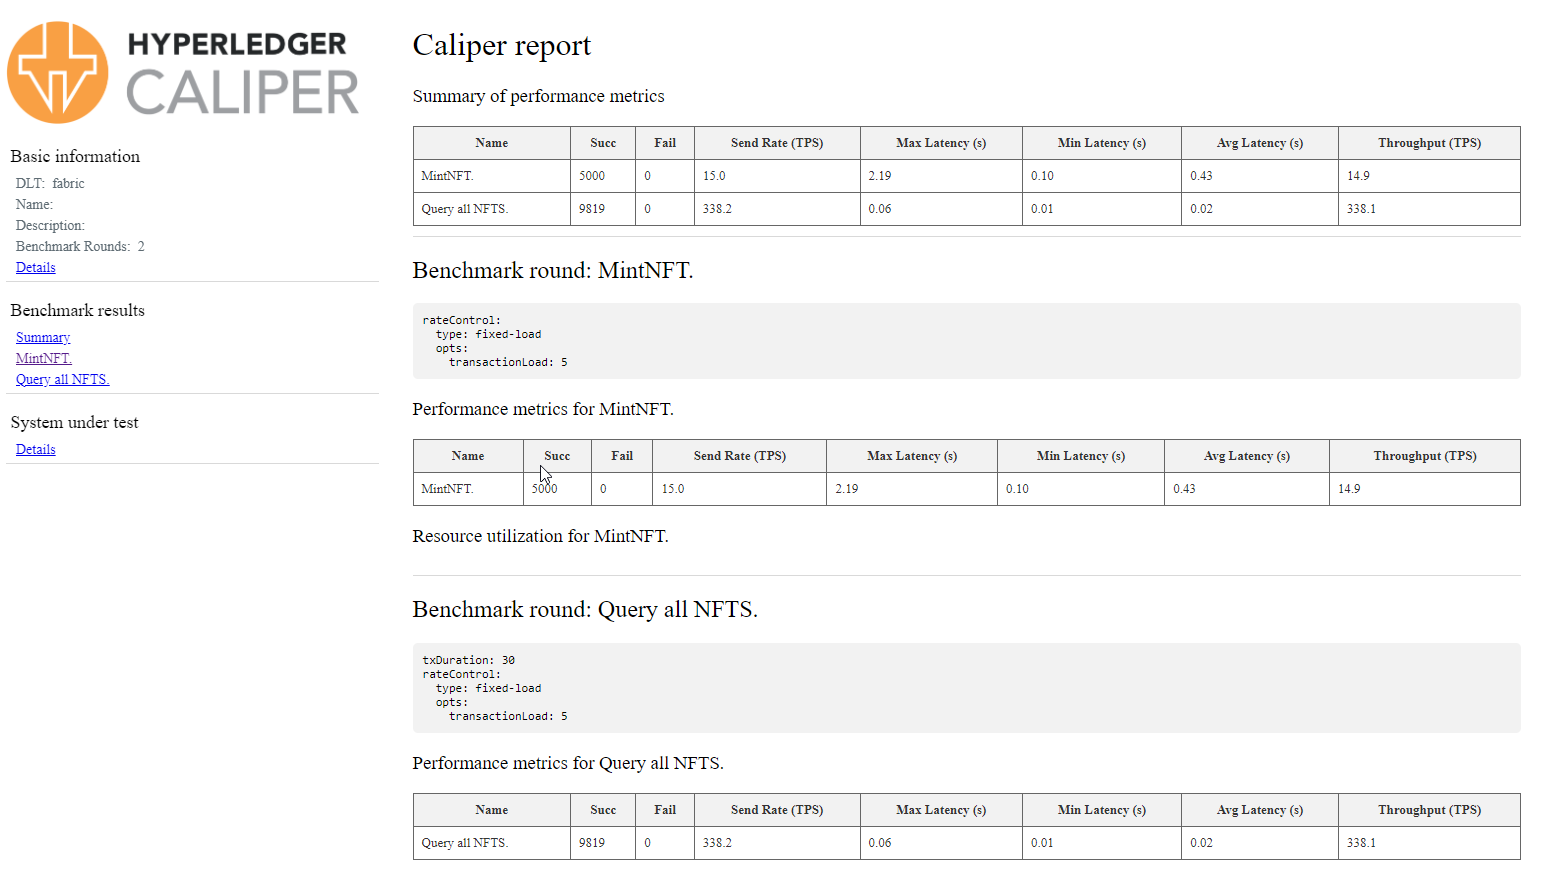
\includegraphics[width=15cm]{img/Caliper.png}
        \caption{Hyperledger Caliper Benchmark results.}
        \label{fig:CaliperBenchmark}
    \end{figure}

\input{chapters/05-conclussions/05-conclusions-00-main}
%-----------------------------------------------------------------
% Now begin the Appendices, including them as separate files

\listoffigures
\listoftables

\appendix
%!TEX root = ../main.tex
\chapter{Code and Instructions}
\label{apx:main}

\section{File repository}
\label{FileRep}
The repository with the code to download the system and perform the simulation is available at:
\url{https://github.com/asahicantu/NFT-Thesis}.
The repository file includes a video sequence showing the sames steps explained in \ref{ch:eval} to perform a simulation.

 \begin{figure}[!h]
        \centering
        \includegraphics[width=5cm]{img/QrCode.png}
        \caption{Qr Code which will redirect to the Github Project stated in \ref{FileRep}}.
        \label{fig:QRCode}
\end{figure}

\section{Instructions to run the code}
To run the project follow the following steps:

\subsection{Prerequisites}
A Linux operating system or bash scripting shell is required.
On a windows machine the usage of \ac{WSL} (any Linux distribution) can help to run the project
Docker Desktop installed (if using Windows with \ac{WSL} make sure the option 'Use WSL 2 Based engine' or similar is selected).

\subsection{Run the application}
\begin{enumerate}
    \item Clone the repository
    \begin{lstlisting}[language=sh]
    git clone https://github.com/asahicantu/NFT-Thesis.git
    \end{lstlisting}
    \item Move to the repository's directory and then to the network directory
    \begin{lstlisting}[language=sh]
    cd NFT-Thesis/network
    \end{lstlisting}
    \item Enable execution mode for all .sh (shell scripting files)
    \begin{lstlisting}[language=sh]
    find . -name "*.sh" -exec chmod +x {} \;
    \end{lstlisting}
    \item Run the network infrastructure
    \begin{lstlisting}[language=sh]
    ./network start
    \end{lstlisting}
    \item Confirm no error occurred
     \begin{figure}[!h]
        \centering
        \includegraphics[width=10cm]{img/Client_Shell.png}
        \caption{Network shell showing successful run}.
        \label{fig:Network_Shell}
    \end{figure}
    \item Run server application in a different terminal
    \begin{lstlisting}[language=sh]
    cd ../web/server && npm install && npm run dev`
    \end{lstlisting}
    \item Confirm no error occurred
     \begin{figure}[!h]
        \centering
        \includegraphics[width=10cm]{img/Server_Shell.png}
        \caption{Server shell showing successful run}.
        \label{fig:Server_Shell}
    \end{figure}
    \item Run web application in a different terminal
    \begin{lstlisting}[language=sh]
    cd ../client && npm install && npm run start`
    \end{lstlisting}
     \item Confirm no error occurred
     \begin{figure}[!h]
        \centering
        \includegraphics[width=10cm]{img/Client_Shell.png}
        \caption{Client shell showing successful run}.
        \label{fig:Client_Shell}
    \end{figure}
    \item Open the application in a web browser by using:
    \url{http://localhost:3000}.
    \item Confirm all steps were properly followed and no error occurred
     \begin{figure}[!h]
        \centering
        \includegraphics[width=10cm]{img/UI_MAIN.png}
        \caption{Main UI Page should be visible}.
        \label{fig:UI_MAIN}
\end{figure}

\end{enumerate}
\newpage
\input{appendices/01-apx-nft}

%-----------------------------------------------------------------
 \backmatter
 \label{Bibliography}
 %\lhead{\emph{Bibliography}}
 % Change the left side page header to "Bibliography"
  \bibliographystyle{unsrtnat}  % Use the "unsrtnat" BibTeX style for formatting the Bibliography
  \bibliography{Bibliography}  % The references (bibliography) information are stored in the file named "Bibliography.bib"

\uisbackcover
\end{document}